% =====================================================================
%  WCCM 2026 — CFRP NDT defect localization with Graph Neural Networks
%  Draft slide deck (Beamer / metropolis).  Build: latexmk -pdf wccm_beamer.tex
%  Figure placeholders point to ../results/ ; swap in final figures before submit.
% =====================================================================
\documentclass[aspectratio=169,10pt]{beamer}

\usetheme{metropolis}
\usecolortheme{default}

\usepackage[T1]{fontenc}
\usepackage[utf8]{inputenc}
\usepackage{booktabs}
\usepackage{amsmath,amssymb}
\usepackage{graphicx}
\usepackage{xcolor}
\usepackage{tikz}
\usetikzlibrary{positioning,arrows.meta}
\usepackage{array}

\definecolor{luhblue}{RGB}{21,101,192}
\definecolor{luhdark}{RGB}{30,30,30}
\definecolor{alertred}{RGB}{198,40,40}
\definecolor{okgreen}{RGB}{27,94,32}

\setbeamercolor{frametitle}{bg=luhblue, fg=white}
\setbeamercolor{progress bar}{fg=luhblue}
\setbeamercolor{alerted text}{fg=alertred}
\setbeamercolor{example text}{fg=okgreen}
\metroset{progressbar=frametitle, block=fill}

\graphicspath{{../results/}{../figures/}}

\newcommand{\best}[1]{{\color{okgreen}\textbf{#1}}}
\newcommand{\bad}[1]{{\color{alertred}#1}}

\title{Graph Neural Networks for Defect Localization\\in Two-Layer CFRP from Ultrasonic NDT}
\subtitle{Architecture study under a balanced noise-augmented recipe}
\author{Keisuke Nishioka \and \textit{[co-authors]}}
\institute{Institute of Continuum Mechanics (IKM), Leibniz Universität Hannover}
\date{WCCM 2026 \quad (draft \today)}

% =====================================================================
\begin{document}

\maketitle
\note{30 min target. Story arc: problem -> data/graph -> imbalance trap ->
recipe -> debugging the collapse -> corrected sweep -> MeshGraphNet wins ->
NEW variants (novelty) -> results -> future (payload + experiments).}

% ---------------------------------------------------------------------
\begin{frame}{Motivation: NDT defect localization in layered CFRP}
\begin{columns}[T]
\begin{column}{0.55\textwidth}
  \vspace{0.3em}
  Carbon-fibre laminates around bolt holes accumulate \textbf{sub-surface
  delaminations} invisible to the eye.

  \vspace{0.8em}
  Ultrasonic NDT yields a per-node response field on a \textbf{two-layer
  mesh} — but reading it by hand is slow and operator-dependent.

  \vspace{0.8em}
  \begin{alertblock}{Goal}
  Predict, for every mesh node, \emph{which of 19 defect classes}
  (incl.\ ``defect-free'') it belongs to — directly from the mesh.
  \end{alertblock}
\end{column}
\begin{column}{0.45\textwidth}
  \centering
  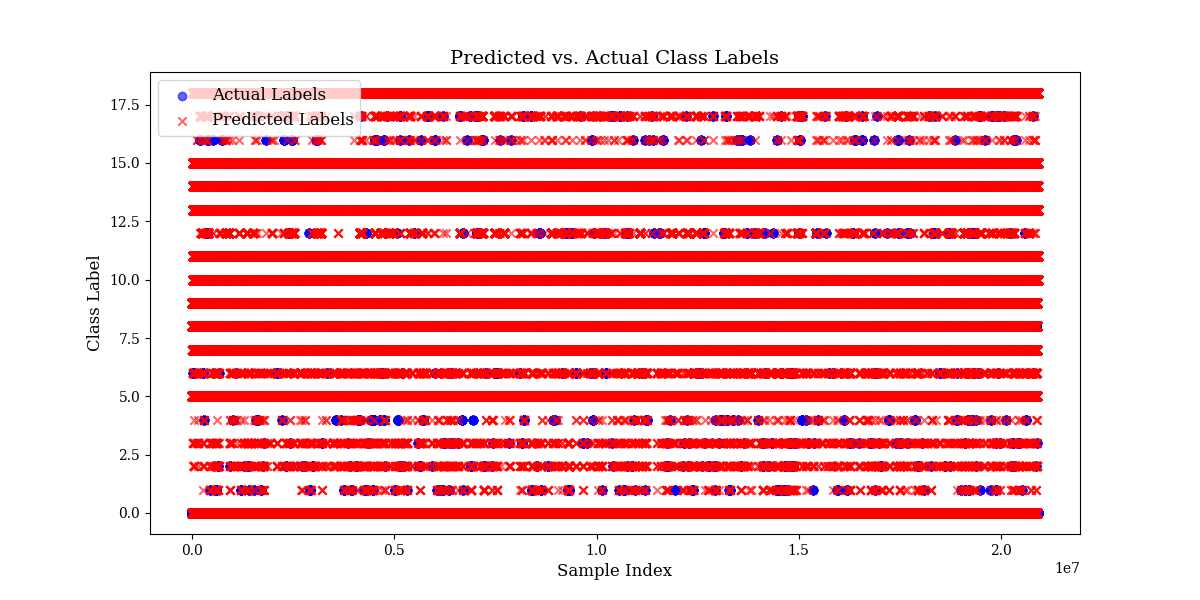
\includegraphics[width=\linewidth]{pred_vs_true_class_labels_20260115_143343.png}\\
  {\scriptsize Predicted vs.\ true node labels on the hole mesh.}
\end{column}
\end{columns}
\end{frame}

% ---------------------------------------------------------------------
\begin{frame}{Data \& graph representation}
\begin{columns}[T]
\begin{column}{0.5\textwidth}
\textbf{One specimen $\rightarrow$ one graph}
\begin{itemize}
  \item $13{,}942$ nodes (two stacked layers around the hole)
  \item Node features: $[x, y, z, \text{DSPSS}]$
  \item Edges: FEM mesh connectivity ($+$ coordinate-difference edge features $[dx,dy,dz,\lVert\cdot\rVert]$)
  \item 19 classes; defect-free is class 0
\end{itemize}
\vspace{0.6em}
\textbf{Input} = \emph{noise-augmented difference} field (damaged $-$ pristine), which isolates the defect signal.
\end{column}
\begin{column}{0.5\textwidth}
\begin{exampleblock}{The trap: extreme imbalance}
Class-0 prior $\approx 0.998$. A model that predicts ``defect-free''
everywhere scores $99.8\%$ accuracy and \bad{macro-F1 $\approx 0$}.
\end{exampleblock}
\vspace{0.4em}
$\Rightarrow$ we report \textbf{macro-F1} and engineer the training
distribution, not just the loss.
\end{column}
\end{columns}
\end{frame}

% ---------------------------------------------------------------------
\begin{frame}{The recipe: balance the data, not (only) the loss}
\begin{enumerate}
  \item \textbf{Noise-augmented difference data} — robustness to acquisition noise.
  \item \textbf{Defect-free negatives (NDF)} — 5000 genuine class-0 graphs added to \emph{train only}.
  \item \textbf{Balanced sampling} — \texttt{--defect\_cap 5000 --ndf\_count 5000} $\to$ 5000:5000.
  \item Leakage control: group-purged val/test split by specimen.
\end{enumerate}
\vspace{0.8em}
\begin{alertblock}{Key finding}
With the recipe in place, the \emph{data distribution dominates}: a faithful
reproduction reaches \textbf{macro-F1 $\approx 0.70$}, vs.\ $\le 0.08$ without it.
\end{alertblock}
\end{frame}

% ---------------------------------------------------------------------
\begin{frame}{A debugging detour: the silent collapse}
\begin{columns}[T]
\begin{column}{0.55\textwidth}
Our refactored trainer \bad{stalled at macro-F1 $\approx 0.16$} across
\emph{every} architecture — while the legacy script reached $0.70$.

\vspace{0.8em}
\textbf{Root cause:} a default-on \texttt{LogitAdjustLoss}\,($\tau{=}1.5$).
On a $0.998$ class-0 prior it \emph{over-boosts} minority classes
$\Rightarrow$ mass over-prediction (high recall, precision $\approx 0$).

\vspace{0.6em}
Fix: \texttt{--no\_logit\_adjust} (Focal loss) $\Rightarrow$ full recovery.
\end{column}
\begin{column}{0.45\textwidth}
\begin{exampleblock}{Lesson}
On extreme imbalance, logit adjustment and class balancing
\emph{compound}. Calibrate the loss to the \emph{already-balanced}
sampler, not the raw prior.
\end{exampleblock}
\end{column}
\end{columns}
\end{frame}

% ---------------------------------------------------------------------
\begin{frame}{Corrected architecture sweep}
\centering
Same recipe, 120 epochs, balanced 5000:5000, group-purged eval.
\vspace{0.6em}

\begin{tabular}{lcl}
\toprule
Architecture & macro-F1 & note \\
\midrule
\best{MeshGraphNet}      & \best{0.764} & Encode-Process-Decode, edge update \\
GATv2                    & 0.694 & dynamic attention \\
GAT (Frontiers baseline) & 0.674 & prior published model ($\sim$0.61) \\
GraphSAGE                & 0.663 & max-aggregation \\
PNA                      & 0.613 & multi-aggregator \\
\bottomrule
\end{tabular}

\vspace{0.8em}
\begin{block}{Takeaway}
Under correct training, the \textbf{mesh-physics architecture
(MeshGraphNet) wins} — beating the legacy GAT recipe (0.70) and the
published baseline (0.61).
\end{block}
\end{frame}

% ---------------------------------------------------------------------
\begin{frame}{Why MeshGraphNet fits the problem}
\begin{columns}[T]
\begin{column}{0.55\textwidth}
\textbf{Encode–Process–Decode} (Pfaff et al., 2021):
\begin{itemize}
  \item node \emph{and} edge embeddings updated at \emph{every}
        message-passing step (residual);
  \item edge feature $=$ coordinate difference $[dx,dy,dz,\text{dist}]$
        $\Rightarrow$ local geometry \& anisotropy;
  \item matches FEM-mesh stress-propagation structure better than
        attention-only GNNs.
\end{itemize}
\end{column}
\begin{column}{0.45\textwidth}
\centering
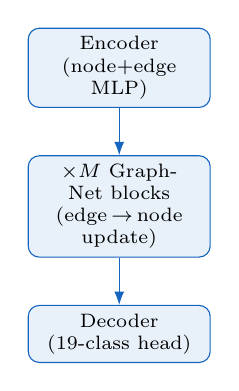
\begin{tikzpicture}[node distance=6mm, every node/.style={font=\scriptsize},
  box/.style={draw=luhblue, fill=luhblue!10, rounded corners, inner sep=3pt, text width=2.1cm, align=center}]
  \node[box] (e) {Encoder\\(node+edge MLP)};
  \node[box, below=of e] (p) {$\times M$ GraphNet blocks\\(edge\,$\to$\,node update)};
  \node[box, below=of p] (d) {Decoder\\(19-class head)};
  \draw[-{Latex}, luhblue] (e)--(p);
  \draw[-{Latex}, luhblue] (p)--(d);
\end{tikzpicture}
\end{column}
\end{columns}
\end{frame}

% ---------------------------------------------------------------------
\begin{frame}{Novelty: four MeshGraphNet variants for layered NDT}
\begin{tabular}{p{2.6cm} p{7.6cm}}
\toprule
Variant & Idea / why it could matter for CFRP \\
\midrule
\textbf{MeshGraphKAN} & Fourier-KAN node encoder — learnable spectral basis
  for the \emph{high-frequency stress-concentration} field (spectral-bias mitigation). \\[2pt]
\textbf{Hybrid-MGN} & mesh edges $+$ \emph{front/back cross-layer ``world'' edges} —
  structurally separates the two laminate layers (no prior work). \\[2pt]
\textbf{BiStride-MGN} & per-graph global-context broadcast — multiscale,
  long-range stress propagation (under-reaching). \\[2pt]
\textbf{MGN-Transformer} & interleaved per-graph self-attention —
  global node interaction. \\
\bottomrule
\end{tabular}
\vspace{0.6em}
\begin{alertblock}{Hypothesis}
\textbf{MeshGraphKAN $\times$ stress concentration} and
\textbf{Hybrid-MGN $\times$ two-layer separation} are the two novel angles
most likely to push past $0.80$.
\end{alertblock}
\end{frame}

% ---------------------------------------------------------------------
\begin{frame}{Variant results \quad {\small[to be filled — runs in progress]}}
\centering
\begin{tabular}{lcl}
\toprule
Variant & macro-F1 & vs.\ MeshGraphNet (0.764) \\
\midrule
MeshGraphNet (baseline) & 0.764 & --- \\
MeshGraphKAN     & \texttt{TBD} & \\
Hybrid-MGN       & \texttt{TBD} & \\
BiStride-MGN     & \texttt{TBD} & \\
MGN-Transformer  & \texttt{TBD} & \\
\bottomrule
\end{tabular}
\vspace{0.8em}

\begin{block}{Target}
Cross the \textbf{0.80} macro-F1 line with a physically-motivated variant.
\end{block}
\end{frame}

% ---------------------------------------------------------------------
\begin{frame}{Per-class performance \& confusion}
\begin{columns}[T]
\begin{column}{0.5\textwidth}
  \centering
  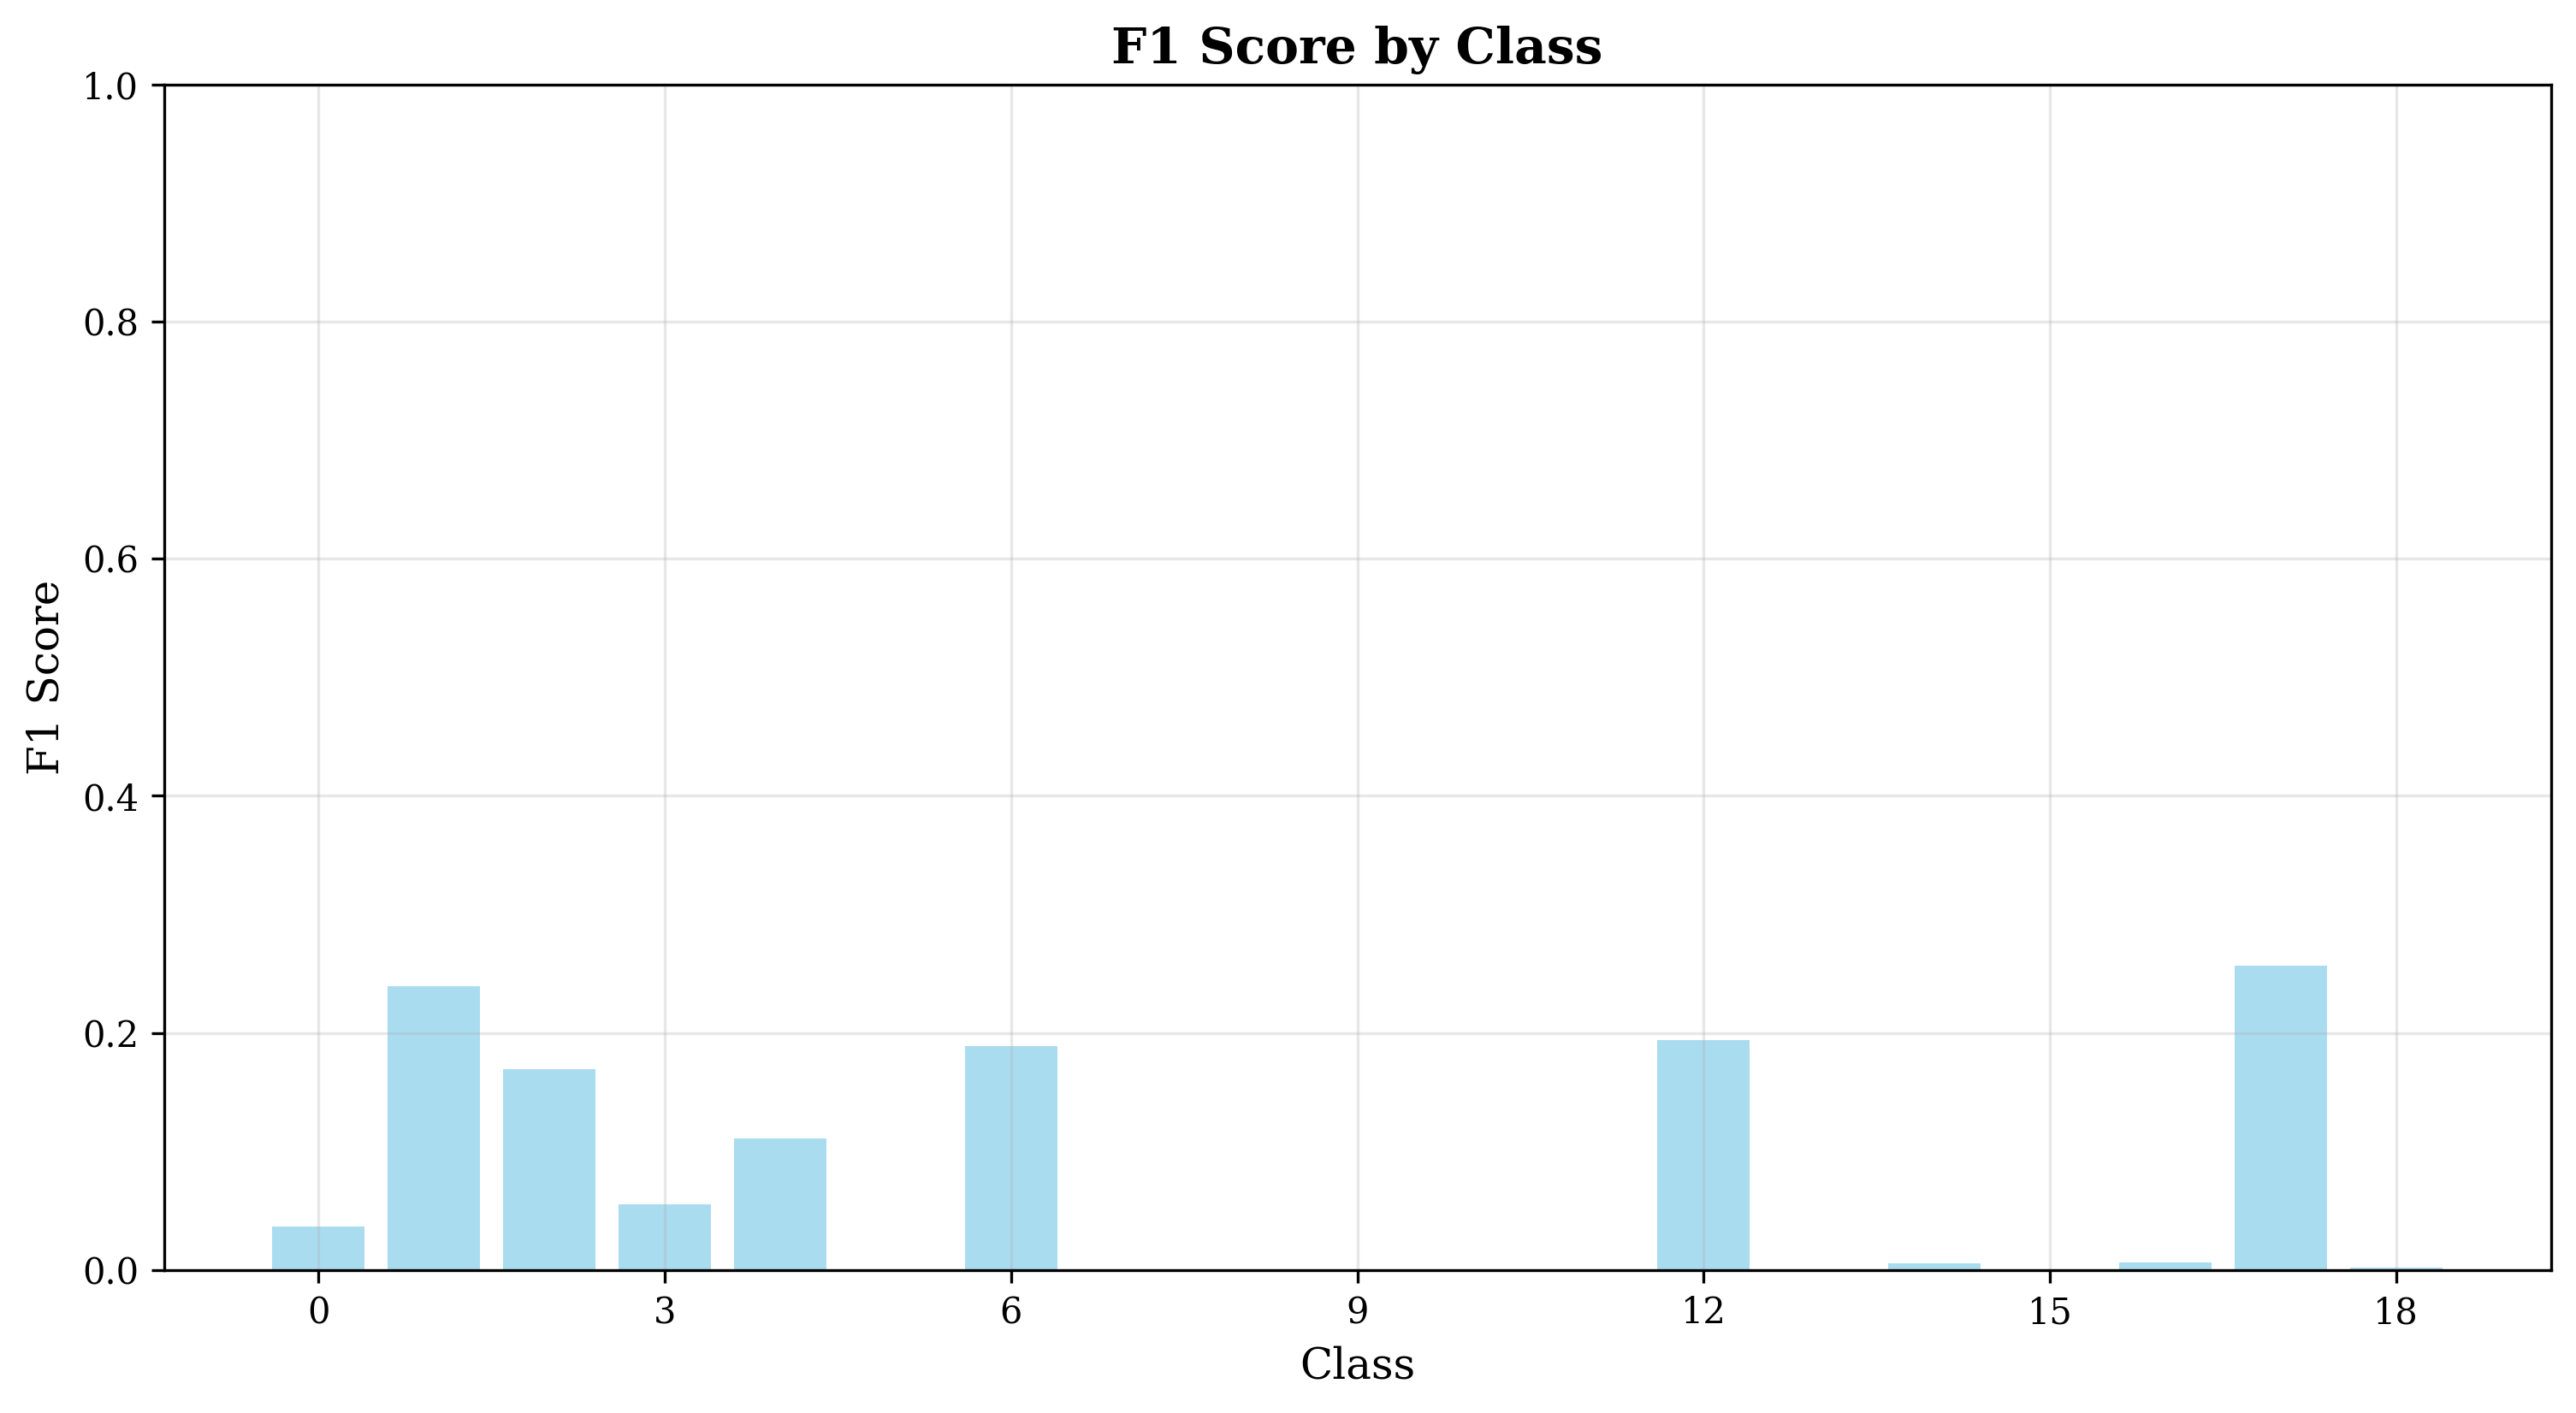
\includegraphics[width=\linewidth]{f1score_class_20260115_143343.png}\\
  {\scriptsize Per-class F1.}
\end{column}
\begin{column}{0.5\textwidth}
  \centering
  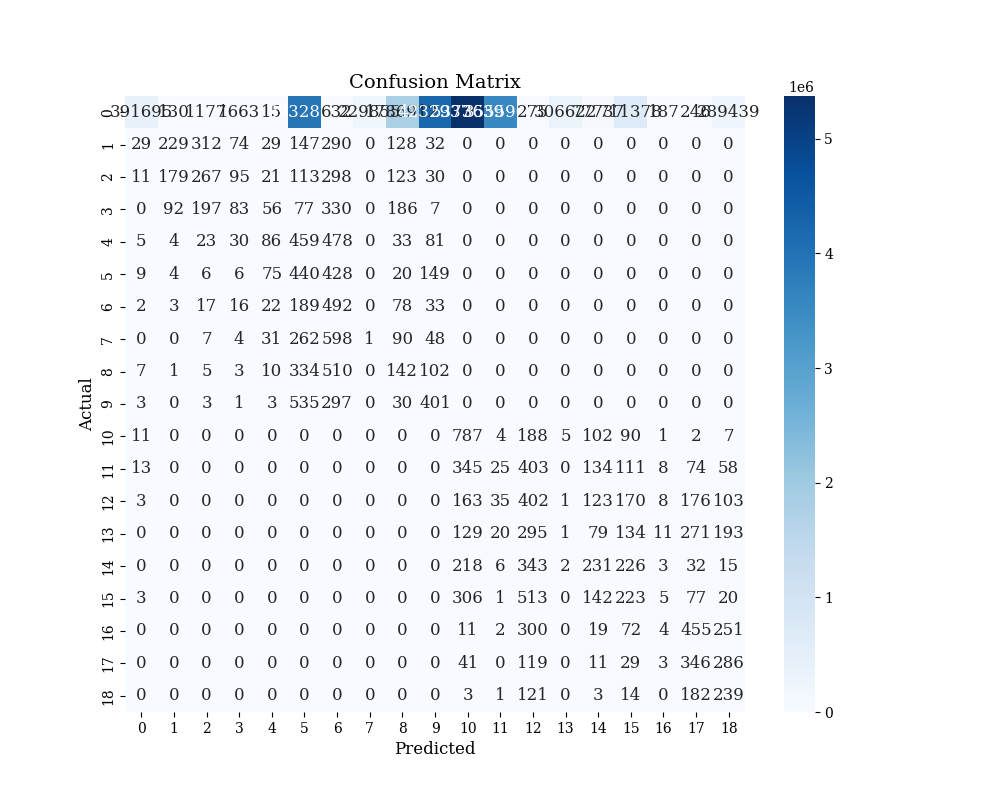
\includegraphics[width=\linewidth]{confusion_matrix_20260115_143343.png}\\
  {\scriptsize Confusion matrix.}
\end{column}
\end{columns}
\end{frame}

% ---------------------------------------------------------------------
\begin{frame}{Conclusions \& outlook}
\begin{itemize}
  \item The \textbf{data recipe} (noise-aug difference $+$ NDF negatives $+$
        balancing) is the dominant factor: $0.08 \to 0.70$.
  \item Under correct training, \textbf{MeshGraphNet} is the best
        architecture (\best{0.764}), beating the published GAT baseline (0.61).
  \item Two \textbf{novel layered-NDT variants} — Fourier-KAN and
        front/back Hybrid edges — target $>0.80$.
\end{itemize}
\vspace{0.6em}
\begin{block}{Future work}
  \begin{itemize}
    \item \textbf{Application:} transfer to aerospace payload-fairing SHM (H3 / GNN-SHM).
    \item \textbf{Validation:} incorporate experimental (non-simulated) NDT data.
  \end{itemize}
\end{block}
\end{frame}

% ---------------------------------------------------------------------
\begin{frame}[standout]
Thank you. \\[0.5em]
{\normalsize Questions?}
\end{frame}

\end{document}
